\documentclass[20pt,a4paper,landscape]{extarticle}
\usepackage[margin=1.45cm,top=0.45cm,left=0.9cm,right=0.9cm,bottom=0.9cm]{geometry}
\usepackage{amsmath}
\usepackage{amssymb}
\usepackage{graphicx}
\usepackage{xcolor}
\usepackage[sfdefault,lf]{FiraSans}
\renewcommand{\familydefault}{\sfdefault}
\setlength{\parindent}{0pt}
\pagestyle{empty}
\everymath{\displaystyle}
\begin{document}
\sffamily
\boldmath
{\LARGE \textbf{Estimating lengths from scale drawings and photos --- Proficient}}\par\vspace{0.45em}
\begin{center}
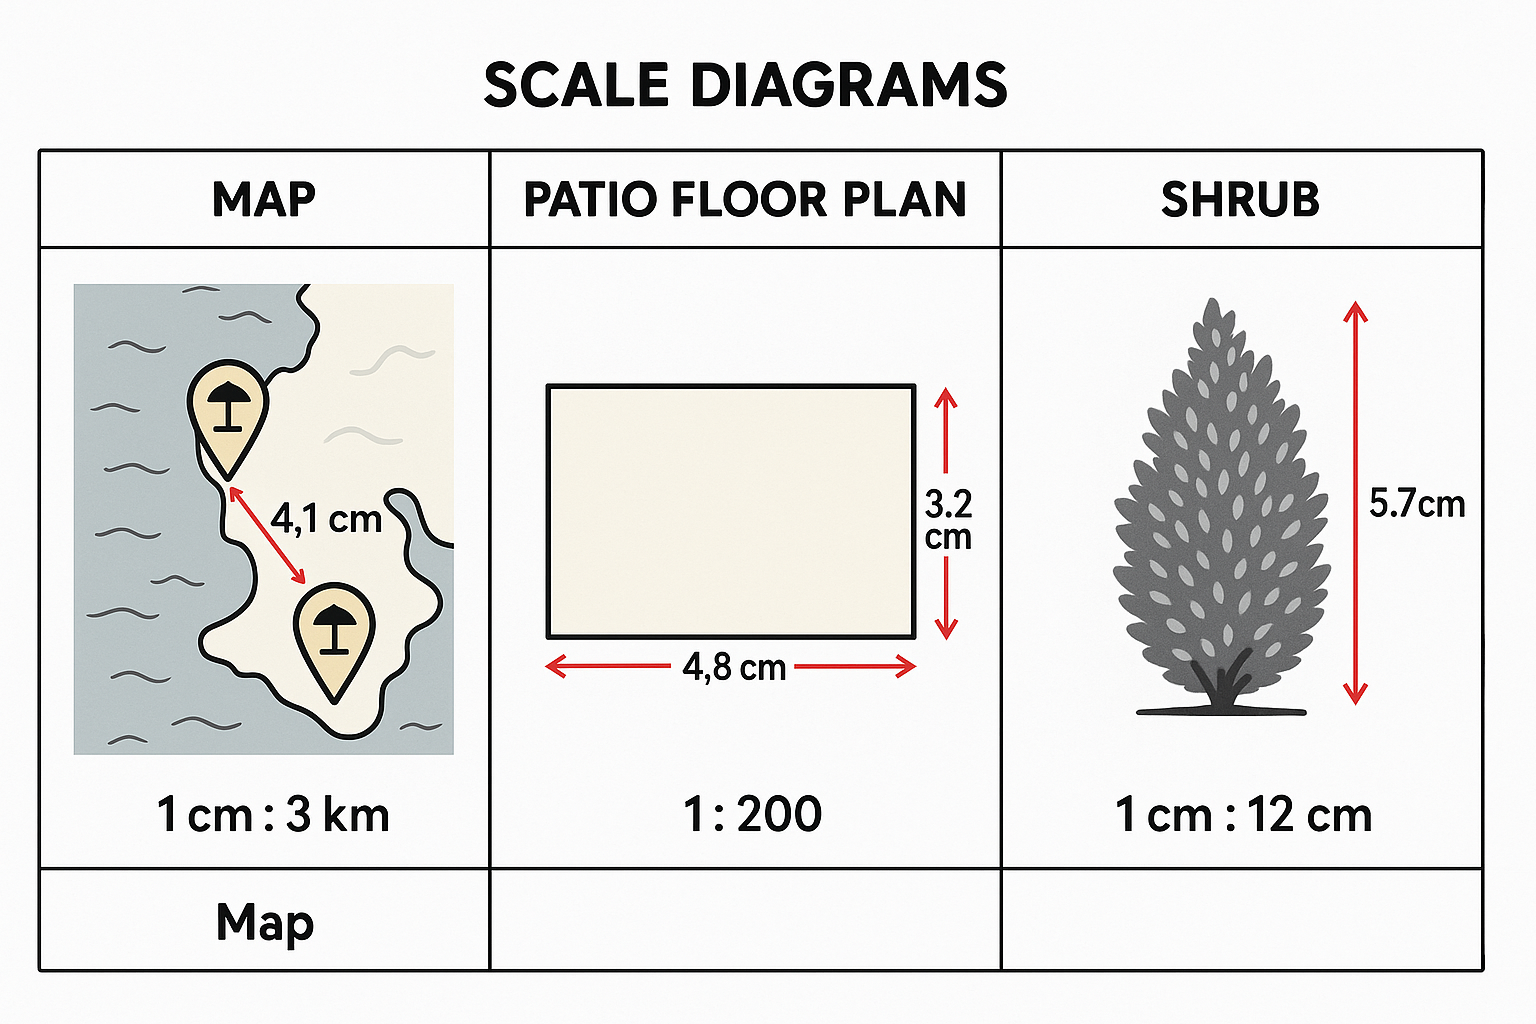
\includegraphics[width=0.94\linewidth,height=0.49\textheight,keepaspectratio]{web-diagrams/proficient-composite.png}
\end{center}
\vspace{0.35em}
\noindent\begin{minipage}[t]{0.275\linewidth}\vspace{0pt}\textbf{1.} Use the map to estimate the real distance between the two marked points. Give your answer in km.\end{minipage}\hspace{0.08\linewidth}\begin{minipage}[t]{0.275\linewidth}\vspace{0pt}\textbf{2.} Use the patio plan to estimate the real dimensions in metres.\end{minipage}\hspace{0.08\linewidth}\begin{minipage}[t]{0.275\linewidth}\vspace{0pt}\textbf{3.} Use the plant measurements to estimate the real plant height in cm.\end{minipage}\par

\vspace{1.0em}
\begin{center}
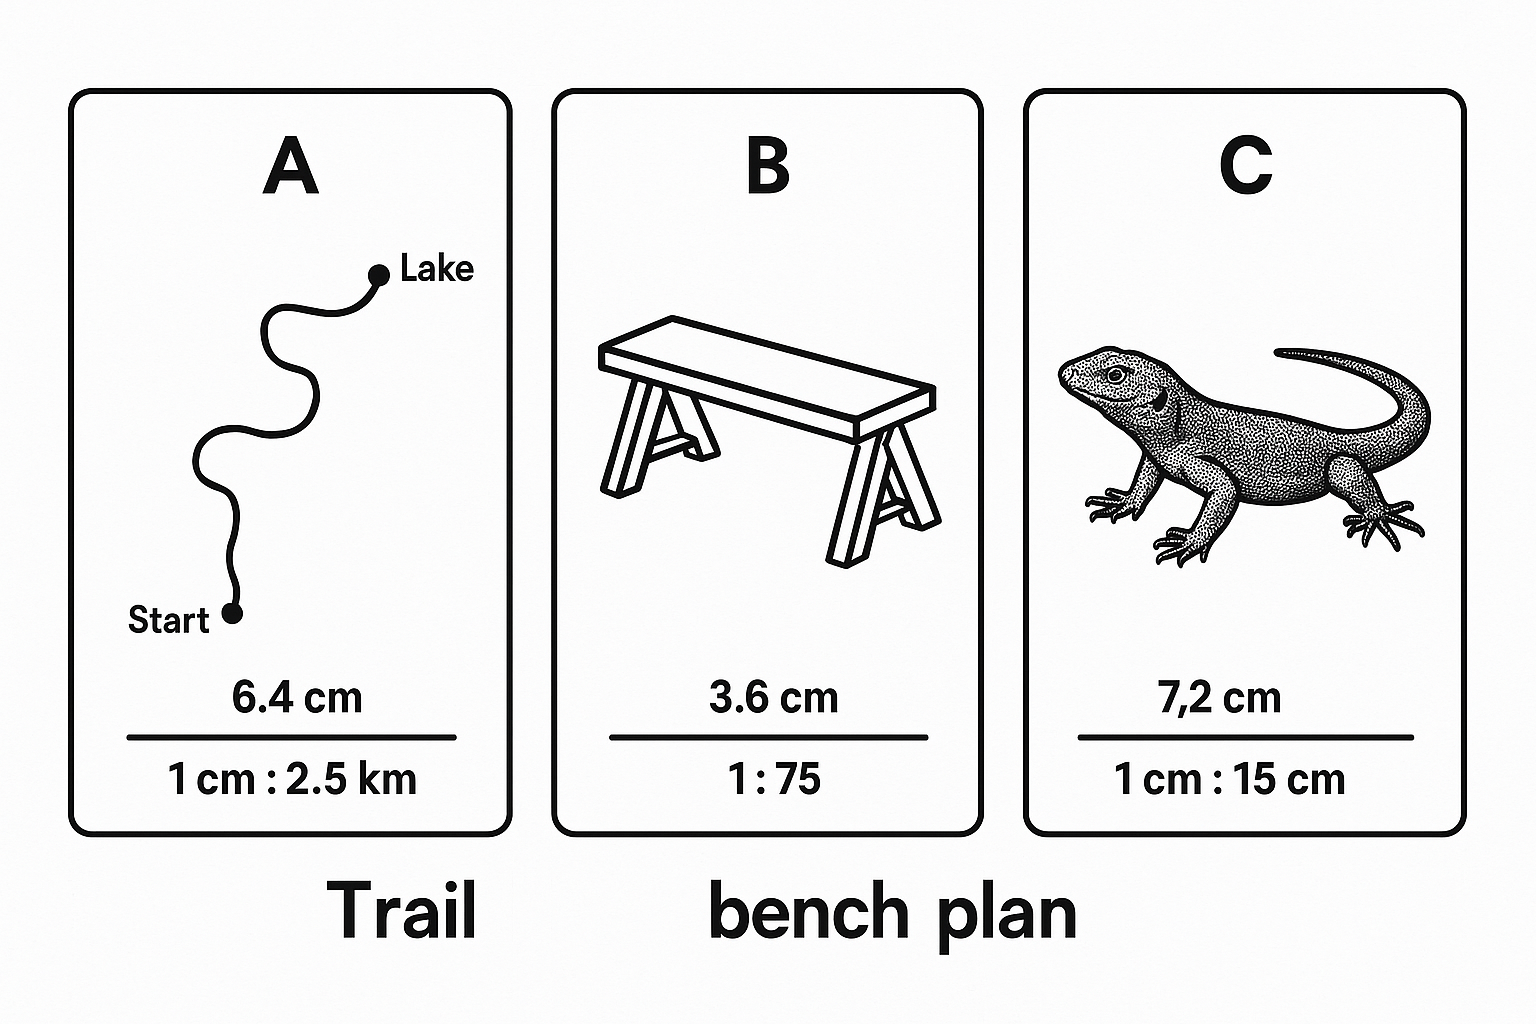
\includegraphics[width=0.94\linewidth,height=0.49\textheight,keepaspectratio]{web-diagrams/proficient-composite-2.png}
\end{center}
\vspace{0.35em}
\noindent\begin{minipage}[t]{0.275\linewidth}\vspace{0pt}\textbf{4.} Use the trail map to estimate the real trail length.\end{minipage}\hspace{0.08\linewidth}\begin{minipage}[t]{0.275\linewidth}\vspace{0pt}\textbf{5.} Use the bench plan to estimate the real bench length in metres.\end{minipage}\hspace{0.08\linewidth}\begin{minipage}[t]{0.275\linewidth}\vspace{0pt}\textbf{6.} Use the lizard measurements to estimate the real lizard length.\end{minipage}\par

\vspace{1.0em}
\noindent\begin{minipage}[t]{0.46\linewidth}\vspace{0pt}\textbf{7.} A scale drawing uses $1:120$. A gate is drawn as $18$ mm wide. Estimate the real width in metres.\end{minipage}\hfill\begin{minipage}[t]{0.46\linewidth}\vspace{0pt}\textbf{8.} A map scale is $1$ cm : $1.5$ km. Two points are $4$ cm apart on the map. Estimate the real distance.\end{minipage}
\end{document}
